\documentclass[Arkitektur/System_main.tex]{subfiles}

\begin{document}
\section{Hardwarearkitektur}

I dette afsnit beskrives hardwarearkitekturen for Beerpong Table. Systemets struktur er illustreret ved hjælp af blokdefinitions diagrammer (BDD). De viser hvordan systemet er sammensat, herunder hvilke dele det består af, og antallet af dele. Et overordnet BDD for systemet er vist i figur \ref{fig:overall_hardware_bdd}. Blokkene og deres funktion er nærmere specificeret i en blokbeskrivelse. Derudover er der lavet et overordnet internt blokdiagram (IBD), som viser bordets grænseflader, og hvordan blokkene er internt forbundet med hinanden. Særligt blokkene Player side og Ball dispenser er essentielle for spillets afvikling. Der er udarbejdet separate diagrammer for disse - Player side er vist i afsnit \ref{sec:playerside_hardware}, mens Ball dispenser kan ses i afsnit \ref{sec:balldispenser_hardware}.

\subsection{Overordnet} \label{sec:overall_hardware}
\subsubsection{Blok definitionsdiagram - \nameref{sec:overall_hardware}}
\begin{figure}[H]
    \centering
    \makebox[\textwidth][c]{%
        \includegraphics[width=1.3\columnwidth,trim={0.24in 0.24in 0.24in 0.24in},clip, page=2]{Arkitektur/graphics/BDD_og_IBD.pdf}
    }
    \caption{Overordnet blok definitionsdiagram for systemet.}
    \label{fig:overall_hardware_bdd}
\end{figure}

\subsubsection{Blokbeskrivelse - \nameref{sec:overall_hardware}}

\begin{table}[H]
\begin{tabular}{L{0.2\columnwidth}|L{0.8\columnwidth}}
\hline
\textbf{Blok} & \textbf{Beskrivelse} \\ \hline
Power Supply & Hele systemet forsynes med en forsyningsspænding. Denne spænding skal laves om til laves om til forskellige spændinger som de forskellige blokke skal bruge. Dette er Power Supply's ansvar.\\ \hline
Player side & Se afsnit \textit{\nameref{sec:systemarkitektur}} \\ \hline
RPi & Se afsnit \textit{\nameref{sec:systemarkitektur}}  \\ \hline
Display & Er placeret i midten af bordet og skal vise information til brugerne. Er forbundet til RPi, og det er vises er styret af den. \\ \hline
Ball dispenser & Se afsnit \textit{\nameref{sec:systemarkitektur}}   \\ \hline
\end{tabular}
\end{table}

\subsubsection{Intern blokdiagram - \nameref{sec:overall_hardware}}

På figur \ref{fig:overall_hardware_ibd} ses et ibd for det overordnede system, hvor signaler er vist.

\begin{figure}[H]
    \centering
    \makebox[\textwidth][c]{%
        \includegraphics[width=1.3\columnwidth,trim={0.24in 0.24in 0.24in 0.24in},clip, page=5]{Arkitektur/graphics/BDD_og_IBD.pdf}
    }
    \caption{Overordnet intern blokdiagram for systemet.}
    \label{fig:overall_hardware_ibd}
\end{figure}

\subsection{Player side} \label{sec:playerside_hardware}
\subsubsection{Blok definitionsdiagram - \nameref{sec:playerside_hardware}}

På figur \ref{fig:playerside_hardware_bdd} ses BDD for player side. Player side findes findes på begge sider af beer pong bordet. Det vil sige at der er en PSoC for hver side af beer pong bordet, sammen med 6 Cup Holders med hver en Cup Light og Cup Sensor.

\begin{figure}[H]
    \centering
    \makebox[\textwidth][c]{%
        \includegraphics[width=1.3\columnwidth,trim={0.24in 0.24in 0.24in 0.24in},clip, page=3]{Arkitektur/graphics/BDD_og_IBD.pdf}
    }
    \caption{Blok definitionsdiagram for Player side.}
    \label{fig:playerside_hardware_bdd}
\end{figure}

\subsubsection{Blokbeskrivelse - \nameref{sec:playerside_hardware}}

\begin{table}[H]
\begin{tabular}{L{0.2\columnwidth}|L{0.8\columnwidth}}
\hline
\textbf{Blok} & \textbf{Beskrivelse} \\ \hline
Cup Holder & Denne blok skal sørge for at lyse under én kop og samtidig detektere om der er en kop eller ej. Den består som det ses på figur \ref{fig:playerside_hardware_bdd} af en Cup light og en Cup sensor \\ \hline
Cup Holders Controller & Denne blok skal sørge for at styre lyset på alle Cup Holders på baggrund af det signal den får fra PSoC Player side. Den skal derudover håndtere signalet fra Cup sensoren i hver Cup Holder og sende ét signal videre til PSoC Player side. \\ \hline
Cup light & Skal lyse under en kop. Styres af PSoC Player side, og ændres alt afhængig af om kop er placeret på den pågældende kopholder og spillets stadie.\\ \hline
Cup sensor & Skal detektere om der er en kop eller ej på et bestem område af bordet (hvor der er plads til én kop)\\ \hline
PSoC Player side & Skal håndtere sensor input fra 6 Cup sensor's og styre lys på 6 Cup light's. Dette skal ske på bagrund af hvad den får at vide fra RPi. Den skal også sende sensor data til RPi\\ \hline
\end{tabular}
\end{table}

\subsubsection{Intern blokdiagram - Cup Holder}
\begin{figure}[H]
    \centering
    \makebox[\textwidth][c]{%
        \includegraphics[width=1.3\columnwidth,trim={0.24in 0.24in 0.24in 0.24in},clip, page=8]{Arkitektur/graphics/BDD_og_IBD.pdf}
    }
    \caption{Intern blokdiagram for Cup Holder.}
    \label{fig:playerside_hardware_bdd}
\end{figure}

\subsubsection{Intern blokdiagram - \nameref{sec:playerside_hardware}}

Nedenfor på figur \ref{fig:playerside_hardware_ibd} ses et ibd for player side, hvor man ser PSoC'en i venstre side, som styre Cup Light i hver Cup Holder vha. Cup Holders Controlelr. Derudover får den også input fra Cup Sensor fra hver Cup Holder, også vha. Cup Holders Controller. PSoC'en styrer så alle Cup Lights afhængig af spillets tilstand og inputter fra alle Cup Sensors. 

\begin{figure}[H]
    \centering
    \makebox[\textwidth][c]{%
        \includegraphics[width=1.3\columnwidth,trim={0.24in 0.24in 0.24in 0.24in},clip, page=6]{Arkitektur/graphics/BDD_og_IBD.pdf}
    }
    \caption{Intern blokdiagram for Player side.}
    \label{fig:playerside_hardware_ibd}
\end{figure}

\subsubsection{Portbeskrivelser - \nameref{sec:playerside_hardware}}

\begin{table}[H]
\begin{tabular}{|L{0.2\textwidth}|L{0.2\textwidth}|L{0.2\textwidth}|L{0.4\textwidth}|}
\hline
\textbf{blok navn}               & \textbf{port navn}     & \textbf{port type}         & \textbf{portbeskrivelse}                                                                     \\ \hline
Player Side             & 5V            & DC                & strømforsyning                                                                       \\ \hline
                        & RPI           & I2C               & kommunikation mellem RPI og player side. protokol beskrevet i grænsefladebeskrivelse \\ \hline
                        & interrupt     & open-drain        & fortæller RPi om hvornår der er nyt data. \\ \hline
PSoC player Side        & lightsControl & SPI               & XXX                                                                                  \\ \hline
                        & irControl     & CMOS              & XXX                                                                                  \\ \hline
                        & sensors       & analog current    & XXX \\ \hline
Cup Holders Controller  & lightsControl & SPI               & XXX \\ \hline
                        & irControl     & CMOS              & XXX \\ \hline
                        & sensorsOutput & analog current    & XXX \\ \hline
                        & lightCtrls    & rgbPWM            & XXX \\ \hline
                        & irCtrls       & CMOS              & XXX \\ \hline
                        & sensors       & analog current    & XXX \\ \hline
Cup Holder              & lightCtrl     & rgbPWM            & XXX \\ \hline
                        & irCtrl        & CMOS              & XXX \\ \hline
                        & sensorsOutput & analog current    & XXX \\ \hline
\end{tabular}
\end{table}

\subsection{Ball dispenser} \label{sec:balldispenser_hardware}
\subsubsection{Blok definitionsdiagram - \nameref{sec:balldispenser_hardware}}

På figur \ref{fig:balldispenser_hardware_bdd} ses et BDD for ball dispenser. Der er kun en ball dispenser i hele systemet. Ball dispenser består af en coin collecter, hvor 5 krone mønten man skal starte spillet med skal indsættes, hvorefter to bolde vil dispenseres. Dette gøres gennem Ball release, der består af en motor(aktuator), som står for dispenseringen. En ting der er vigtig for systemet er at vide, hvornår der er nok bolde i ball dispenseren. Dette gøres ved hjælp af underblokken ball count sensor. Her vil en sensor sørge for at der er mindst to bolde klar til dispensering hele tiden ellers lyser en status LED rødt. Hertil vil en status LED lyse grønt, hvis ball dispenseren er fuld. Samspil mellem alle blokkene styres af PSoC'en.

\begin{figure}[H]
    \centering
    \makebox[\textwidth][c]{%
        \includegraphics[width=1.3\columnwidth,trim={0.24in 0.24in 0.24in 0.24in},clip, page=4]{Arkitektur/graphics/BDD_og_IBD.pdf}
    }
    \caption{Blok definitionsdiagram for Ball dispenser.}
    \label{fig:balldispenser_hardware_bdd}
\end{figure}

\subsubsection{Blokbeskrivelse - \nameref{sec:balldispenser_hardware}}

\begin{table}[H]
\begin{tabular}{L{0.2\columnwidth}|L{0.8\columnwidth}}
\hline
\textbf{Blok} & \textbf{Beskrivelse} \\ \hline

Coin collector & Skal detektere når der indsættes mønter. Den skal detektere 5kr mønter og andre skal returneres til brugeren. Derudover skal 5kr mønten også returneres hvis systemet ikke er i en tilstand hvor det er klar til at modtage mønter. Fx at der er et spil i gang eller hvis der ikke er flere bolde.\\ \hline
Ball count sensor & Skal holde styr på hvor mange bolde der er i dispenseren\\ \hline
Ball release & Skal sørge for at levere en/flere bold(e) til brugeren\\ \hline
Actuator & Skal lave bevægelsen der leverer en bold \\ \hline
Actuator sensor & Skal detektere positionen af Actuator. Dette bruges til at styre Actuator.\\ \hline
Actuator controller & Skal styre Actuator.\\ \hline
PSoC ball dispenser & Skal håndtere sensor input fra Coin collector. Og skal afhængig af information modtaget fra RPi styre om Coin collector skal returnere mønter. Den skal også få Ball release til at levere en bold når den får det at vide af RPi. Derudover skal den også fortælle RPi om hvor mange bolde der er tilbage. \\ \hline
Status LEDs & To LED'er til at informere om bold dispenseren er fuld eller tom. En rød LED lyser når den er tom (under 2 bolde tilbage) og en grøn LED lyser når bolddispenseren er fuld\\ \hline
\end{tabular}
\end{table}

\subsubsection{Intern blokdiagram - \nameref{sec:balldispenser_hardware}}

På figur \ref{fig:balldispensere_hardware_ibd} ses et ibd diagram for Ball dispenseren, hvor man her ser, at PSoC'en har kontakt til Raspberry pie, og sørger for samspillet mellem coincollector, Ball count sensor og motoren aktuator. Man kan her se at ball release blokken ikke længere er med fra BDD diagrammet. Derimod er de blokke den bestod af med, som er aktuatoren(den bevægelige del), en actuator controller til styring af den bevægelige motor og til sidst en sensor til at holde styr på motorens(aktuatorens) position.

\begin{figure}[H]
    \centering
    \makebox[\textwidth][c]{%
        \includegraphics[width=1.3\columnwidth,trim={0.24in 0.24in 0.24in 0.24in},clip, page=7]{Arkitektur/graphics/BDD_og_IBD.pdf}
    }
    \caption{Intern blokdiagram for Ball dispenser.}
    \label{fig:balldispensere_hardware_ibd}
\end{figure}

\subsubsection{Port beskrivelse - Ball dispenser}

\begin{table}[]
\begin{tabular}{|l|l|l|l|}
\hline
blok navn                            & port navn         & port type & port beskrivelse                                                                          \\ \hline
\multirow{3}{*}{Ball dispenser}      & 5V                & DC        & strømforsyning til psoc mm.(se ibd for playerside)                                        \\ \cline{2-4} 
                                     & 12V               & DC        & strømforsyning til actuator controller                                                    \\ \cline{2-4} 
                                     & RPI               & I2C       & I2C protocol er beskrevet i grænseflade beskrivelse                                       \\ \hline
\multirow{7}{*}{Psoc Ball dispenser} & Actuator Feedback & XXX       & XXX                                                                                       \\ \cline{2-4} 
                                     & acceptCoins       & XXx       & XXX                                                                                       \\ \cline{2-4} 
                                     & CoinSensor        & XXX       & XXX                                                                                       \\ \cline{2-4} 
                                     & ballcount         & XXX       & XXX                                                                                       \\ \cline{2-4} 
                                     & emptyLed          & bool      & høj(\textgreater{}2V) når der ikke er minimum to bolde i dispenseren. Lav(\textless{}0.8) \\ \cline{2-4} 
                                     & fullLed           & bool      & Er høj(\textless{}2V) når dispenseren er fuld. Lav(\textless{}0.8)                        \\ \cline{2-4} 
                                     & ballControl       & XXX       & XXX                                                                                       \\ \hline
coin collecter                       & coinSignal        & XXX       & XXX                                                                                       \\ \hline
Ball count sensor                    & ballCount         & XXX       & XXX                                                                                       \\ \hline
\multirow{2}{*}{status LEDs}         & empty             & bool      & høj(\textgreater{}2V) når der ikke er minimum to bolde i dispenseren. Lav(\textless{}0.8) \\ \cline{2-4} 
                                     & full              & bool      & Er høj(\textless{}2V) når dispenseren er fuld. Lav(\textless{}0.8)                        \\ \hline
Actuator                             & control           & XXX       & XXX                                                                                       \\ \hline
Actuator controller                  & actuatorControl   & XXX       & XXX                                                                                       \\ \hline
Actuator sensor                      & feedback          & XXX       & XXX                                                                                       \\ \hline
\end{tabular}
\end{table}

\end{document}